%%%%%%%%%%%%%%%%%%%%%%%%%%%%%%%%%%%%%%%%%
% University Assignment Title Page 
% LaTeX Template
% Version 1.0 (27/12/12)
%
% This template has been downloaded from:
% http://www.LaTeXTemplates.com
%
% Original author:
% WikiBooks (http://en.wikibooks.org/wiki/LaTeX/Title_Creation)
%
% License:
% CC BY-NC-SA 3.0 (http://creativecommons.org/licenses/by-nc-sa/3.0/)
% 
% Instructions for using this template:
% This title page is capable of being compiled as is. This is not useful for 
% including it in another document. To do this, you have two options: 
%
% 1) Copy/paste everything between \begin{document} and \end{document} 
% starting at \begin{titlepage} and paste this into another LaTeX file where you 
% want your title page.
% OR
% 2) Remove everything outside the \begin{titlepage} and \end{titlepage} and 
% move this file to the same directory as the LaTeX file you wish to add it to. 
% Then add \input{./title_page_1.tex} to your LaTeX file where you want your
% title page.
%
%%%%%%%%%%%%%%%%%%%%%%%%%%%%%%%%%%%%%%%%%

\documentclass[12pt,a4paper]{article}
\usepackage[english]{babel}
\usepackage[utf8x]{inputenc}
\usepackage{amsmath}
\usepackage{graphicx}
\usepackage[colorinlistoftodos]{todonotes}
\usepackage{url}
\usepackage[section]{placeins}

\begin{document}

\begin{titlepage}

\newcommand{\HRule}{\rule{\linewidth}{0.5mm}}

\center

\textsc{\LARGE Coursera}\\
\textsc{\large The Hong Kong University of Science and Technology}\\[1cm]
\textsc{\Large Full Stack Web Development Specialization}\\[0.5cm]
\textsc{\large Capstone Project}\\[0.5cm]

\HRule \\[0.4cm]

\includegraphics[width=.5\paperwidth]{fig/mymovies.png}
\HRule \\[1cm]
 

\begin{minipage}{0.4\textwidth}
\begin{flushleft} \large
\emph{Author:}\\
Tiago \textsc{Justino}
\end{flushleft}
\end{minipage}
~
\begin{minipage}{0.4\textwidth}
\begin{flushright} \large
\emph{Supervisor:} \\
Jogesh \textsc{Muppala}
\end{flushright}
\end{minipage}\\[1cm]


{\large \today}\\[1cm]

\vfill

\includegraphics[width=.2\paperwidth]{fig/coursera.png}
\hspace{2cm}

\includegraphics[width=.2\paperwidth]{fig/hkust.png}

\end{titlepage}
%----------------------------------------------------------------------------------------

\section{Introduction}

MyMovies is a social network for cinema fans. It keeps track of movies you've
watched, want to watch and don't want to watch. By leveraging the IMDB database
it allows you to add custom pieces of information, such as, rating and
comments. Also, the social network aspect brings you the possibility of
discovering new movies you want to watch and new points of view on movies
you've watched at the same time that it allows you to share good moments with
people you love.

As a bonus, by keeping track of people's movie watching habits MyMovies is able
to help the cinema industry on targeting their customer more precisely.

\subsection{Expected List of Features}

Inside the scope of this project we plan on achieving the following features:

\begin{itemize}
  \item The user will be able to create an account and login to the system with
    or without Facebook. The user will also be able to link or unlink their
    MyMovies account to their Facebook account;
  \item The user will be able to invite other users to be their friends on
    MyMovie. The invited user will be able to accept or decline the invite;
  \item The user will be able to invite their Facebook friends to join
    MyMovies.
  \item The user will be able to follow other users. Users added as friends are
    followed by default. The user will also be able unfollow friend without
    unfriending them;
  \item The user will be able to mark a movie as watching,
    watched, want to watch or don't want to watch;
  \item For movies previously marked as watched, the user will be able to
    favorite and to add rating and comments;
  \item The user will be able to \textit{fan} names, such as actors, actresses,
    directors and producers;
  \item Movies marked as watching are automatically marked as watched after the
    movie duration (known from imdb api);
  \item When marking a movie as watching or watched the user will be able to
    mark a friend as "watching with";
  \item The user will be able to add a date (day, month or year) for movies
    watched in the past. Date is not mandatory;
  \item The user will be able to mark a movie as watched more than once;
  \item The user will be able to access a timeline page where they can see the
    activities of whom they follow. The timeline will show activities such as
    watching and watched movies, and comments;
  \item The user will be able to like or comment on friend's activities,
  \item The user will be able to mark their comment (or part of it) as spoiler,
  \item Comments marked as spoiler will appear with a warning message on a user
    timeline if they haven't watched that movie,
  \item The user will be able to create and join groups (private and public),
    such as "Movie Club at Work" or "Stanley Kubrick Fans",
  \item The user will be able to recommend a movie to a friend.
\end{itemize}

\section{Design and Implementation}

Initially only three of the planned features were actually implemented: Login,
search for movie title, and add and remove to/from watched list. The three
screens can be seen at Figures \ref{fig:login}, \ref{fig:search} and
\ref{fig:profile};

The application scaffolding was done using a github tutorial \cite{githubtuto}
which serves both the front-end and back-end together.

\subsection{Front-end}

The front-end was implemented using AngularJS version 1.4.5 together with
Bootstrap 3.3.5 and Angular-Route. Also, a client service for accessing the
Omdb API was implemented here (see Section \ref{sec:omdb} for more details).

The routes are:

\begin{description}
  \item[home:] Shows the search page (Figure \ref{fig:search}) if the user is
    logged in. If the user is not logged in, it redirects to the login/signup
    page (Figure \ref{fig:login}).
  \item[login:] The login/signup page.
  \item[profile:] The profile page. Shows the watched movies list.
\end{description}

\subsection{Back-end}

The back-end was implemented using Express 4.13, Mongoose 4.3 and Passport 0.3.

The exposed endpoints are:

\begin{description}
  \item[login (post):] Checks the user credentials and authenticate them.
  \item[logout (post):] Destroys the user session.
  \item[loggedin (get):] Returns the user info if they're loggedin.
  \item[signup (post):] Registers a new user.
  \item[watched (post):] Adds a movie to the watched list.
  \item[watched/:id (delete):] Removes a movie from the watched list.
\end{description}

\subsection{Omdb API} \label{sec:omdb}

The initial idea was using Imdb to retrieve the movies information.
Unfortunately, Imdb doesn't provide any official API. There is, however, an
unofficial API called Omdb (The Open Movie Database, \cite{omdb}). This API
provides not just information from IMDB, but from other movie websites such as
rottentomatoes.com.

Here we opted out for keeping the API access only on the client side, the
reason being bandwidth saving.

\begin{figure}[!htb]
\centering
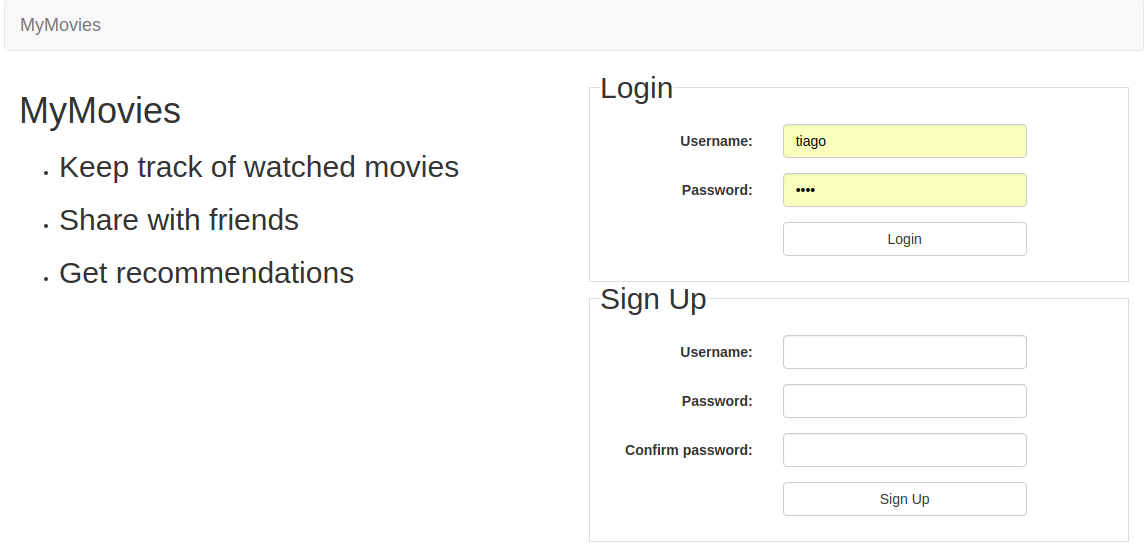
\includegraphics[width=0.8\textwidth]{fig/01-login.png}
\caption{\label{fig:login}Sign up / Login page.}
\end{figure}

\begin{figure}[!htb]
\centering
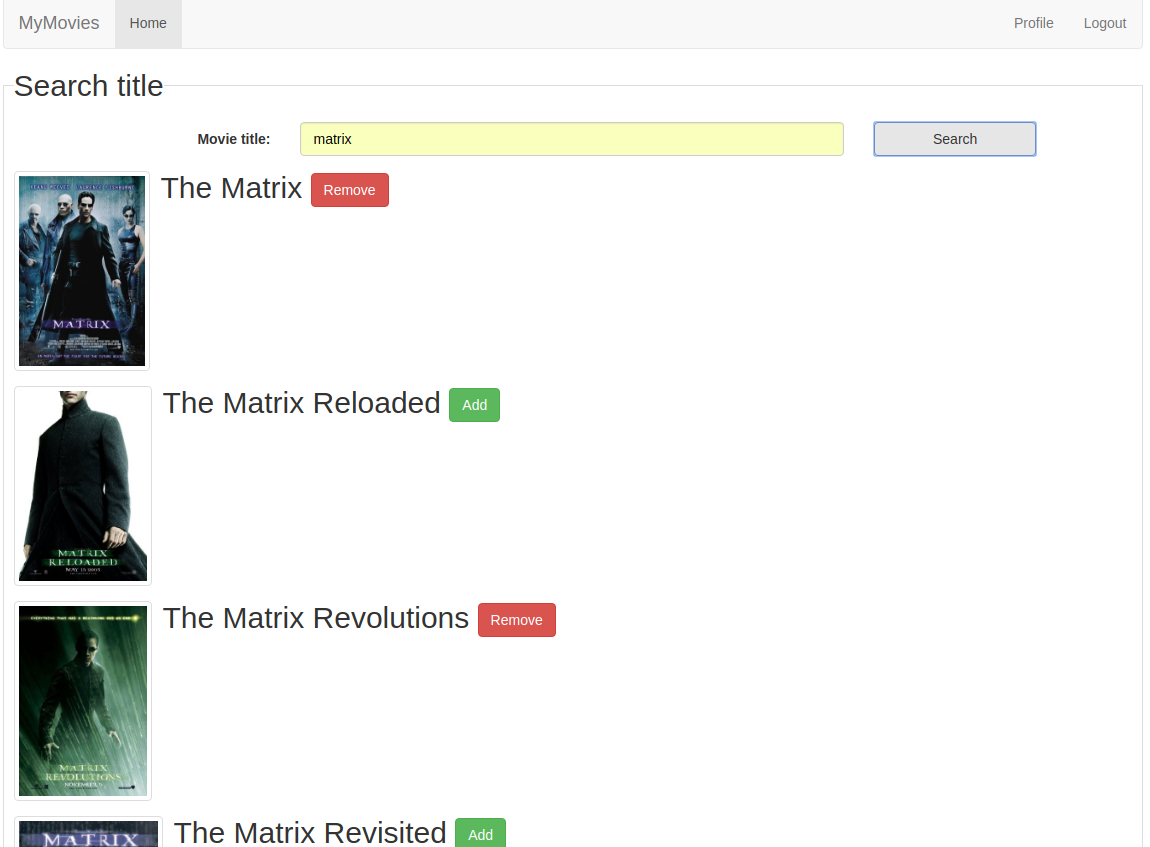
\includegraphics[width=0.8\textwidth]{fig/02-search.png}
\caption{\label{fig:search}Search for titles.}
\end{figure}


\begin{figure}[!htb]
\centering
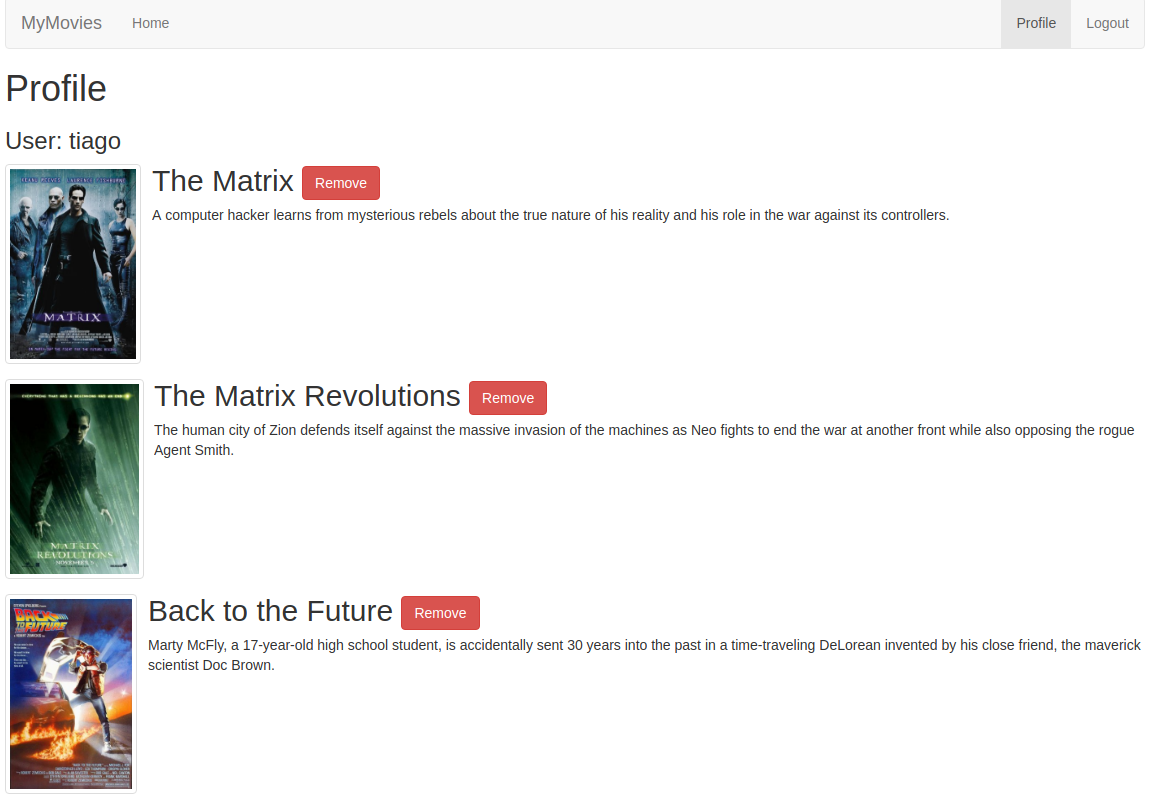
\includegraphics[width=0.8\textwidth]{fig/03-profile.png}
\caption{\label{fig:profile}Profile page.}
\end{figure}

\section{Conclusion}

The results were much less than expected due mainly to two reasons: 1. I
believe I planed too many features to be done in two weeks. and 2. I
underestimated the difficulty of using the Imdb unofficial API.

\bibliographystyle{plain}
\bibliography{bib}

%\label{sec:examples}
%
%\todo{Here's a comment in the margin!}
%\todo[inline, color=green!40]{This is an inline comment.}
%
%\begin{figure}
%\centering
%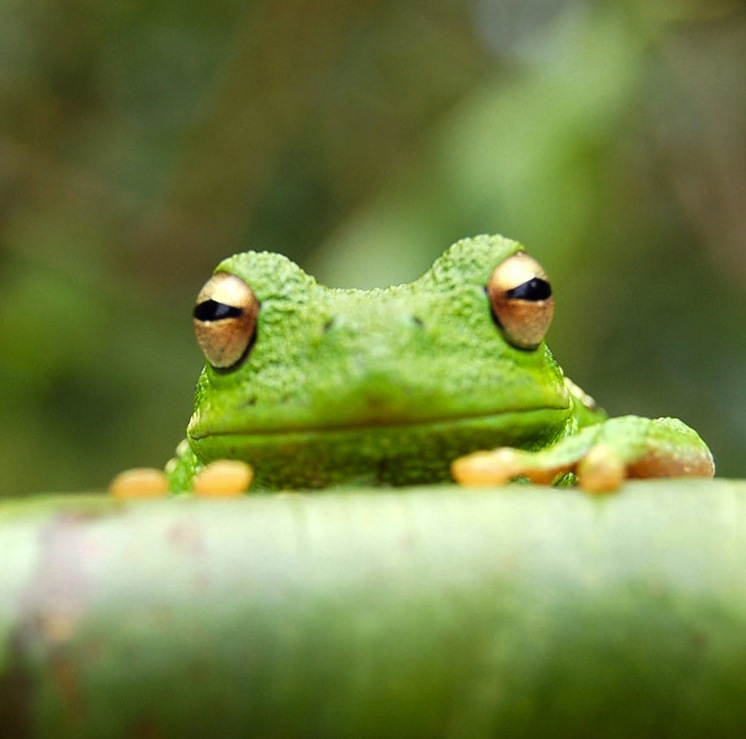
\includegraphics[width=0.5\textwidth]{frog.jpg}
%\caption{\label{fig:frog}This is a figure caption.}
%\end{figure}
%
%\begin{table}
%\centering
%\begin{tabular}{l|r}
%Item & Quantity \\\hline
%Widgets & 42 \\
%Gadgets & 13
%\end{tabular}
%\caption{\label{tab:widgets}An example table.}
%\end{table}
%
%\dots
%
%\begin{enumerate}
%\item Like this,
%\item and like this.
%\end{enumerate}
%\dots or bullet points \dots
%\begin{itemize}
%\item Like this,
%\item and like this.
%\end{itemize}

\end{document}
